\section{Übung 1 - Jahresabschlussanalyse, Working Capital Management, Cash Management}

\textbf{Ziele des Financial Management}:
\begin{center}
	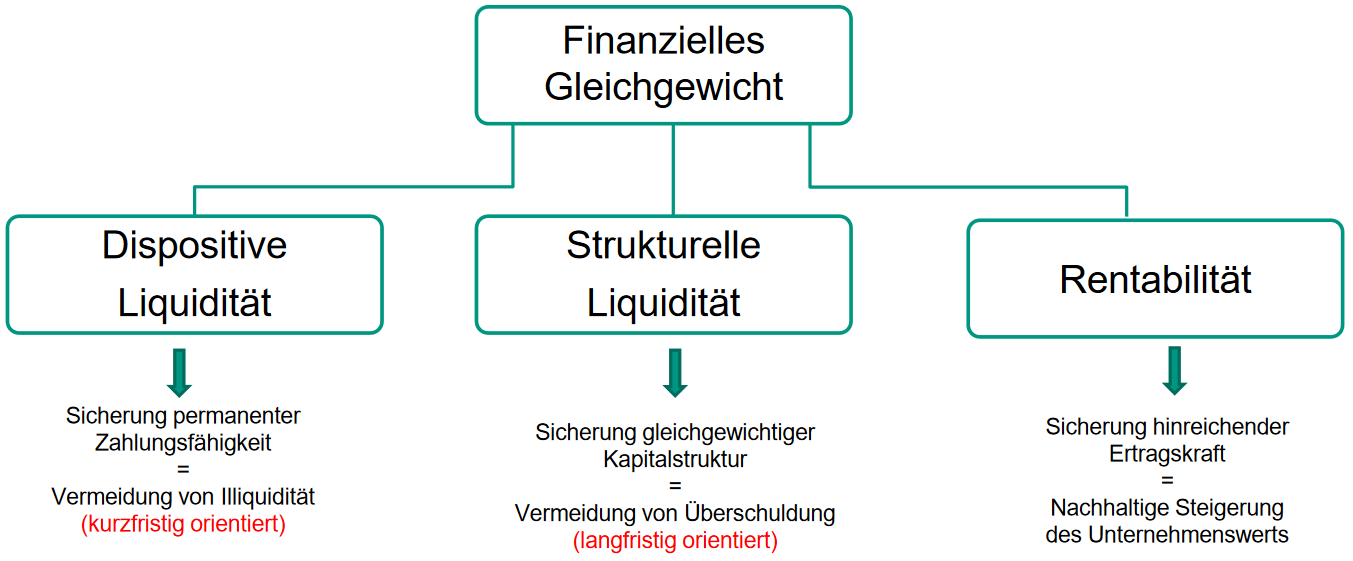
\includegraphics[width=0.8\textwidth]{images/e1.png}
\end{center}

\textbf{Elemente des Jahresabschlusses}:
\begin{itemize}
	\item \textbf{Kernelemente}: GuV, Bilanz, Kapitalflussrechnung
	\item \textbf{Weitere Elemente}: Eigenkapitalveränderungsrechnung, Management Discussion and Analysis, Anhang
\end{itemize}

\textbf{Gewinn- und Verlustrechnung}: Listet Erlöse und Kosten eines Unternehmens über einen bestimmten Zeitraum auf

\textbf{Bilanz}: Zeigt welche Vermögensgegenstände ein Unternehmen besitzt (Aktiva) und wie die Vermögensgegenstände finanziert sind (Passiva)
\begin{center}
	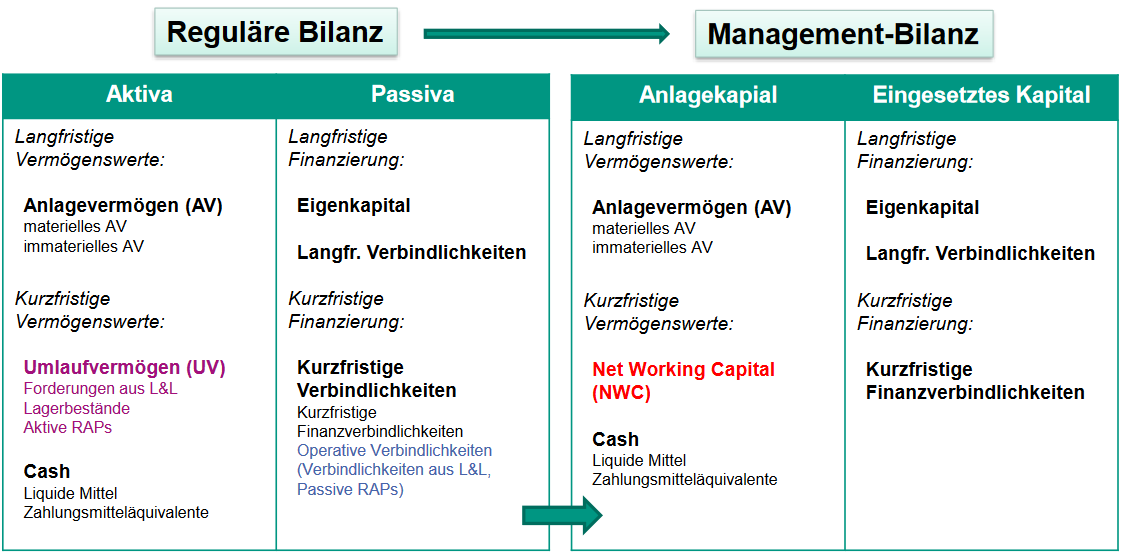
\includegraphics[width=\textwidth]{images/e2.png}
\end{center}
$\text{NWC} = \text{Umlaufvermögen} – \text{operative Verbindlichkeiten}$
\pagebreak

\textbf{Kapitalflussrechnung}: 
\begin{itemize}
	\item Führt Informationen aus der GuV und Bilanz zusammen $\rightarrow$ Wie viele Barmittel hat ein Unternehmen erwirtschaftet hat und wofür werden diese verwendet?
	\item Unterteilt in Cash Flow aus operativer Tätigkeit, Investitionstätigkeit und Finanzierungstätigkeit
\end{itemize}

\textbf{Ziele der Jahresabschlussanalyse}:
\begin{itemize}
	\item Erhöhung der Aussagekraft des Jahresabschlusses
	\item Erleichterung der Beurteilung der Vermögens-, Finanz- und Ertragslage des Unternehmens
	\item Vergleich eines Unternehmens mit sich selbst über den Zeitablauf oder mit anderen Unternehmen
\end{itemize}

\subsection{Kennzahlen Jahresabschlussanalyse}
\textbf{Liquidität}:
\begin{itemize}
	\item Liquidität 1. Grades (Cash Ratio) $=\cfrac{\text{liquide Mittel}}{\text{ kurzfristige Verbindlichkeiten}}$	
	\item Liquidität 2. Grades (Quick/Acid Test Ratio) $=\cfrac{\text{liquide Mittel}+\text{kurzfristige Forderungen}}{\text{kurzfristige Verbindlichkeiten}}$
	\item Liquidität 3. Grades (Current Ratio) $=\cfrac{\text{UV}}{\text{kurzfristige Verbindlichkeiten}}$ \\($\geq 2$, Bankers' Rule)
	\item Zinsdeckungsrate (Interest Coverage Ratio) $=\cfrac{\text{EBIT}}{\text{Zinsaufwand}}$
\end{itemize}
	
\textbf{Working Capital:}
\begin{itemize}
	\item Working Capital (WC) $=(\text{UV} -\text{liquide Mittel} -  \text{kurzfristige finanzielle Vermögenswerte})$	
	\item Net Working Capital (NWC) $=\text{WC}-(\text{kurzfristige Verbindlichkeiten}-\text{kurzfristige Finanzverb.})$
	\item Net Working Capital Ratio $=\cfrac{\text{NWC}}{\text{Umsatz}}$
\end{itemize}

\textbf{Anlagendeckung:}
\begin{itemize}
	\item Anlagendeckungsgrad 1 $=\cfrac{\text{EK}}{\text{AV}}\qquad (\geq 1$, Goldene Bilanzregel, strenge Form)
	\item Anlagendeckungsgrad 2 $=\cfrac{\text{EK}+\text{langfristige Verbindlichkeiten}}{\text{AV}}$\\ ($\geq 1$, Goldene Bilanzregel, milde Form)
\end{itemize}

\textbf{Vermögensstruktur:}
\begin{itemize}
	\item Anlagenintensität $=\cfrac{\text{AV}}{\text{Gesamtkapital (Bilanzsumme)}}$
\end{itemize}
	
\textbf{Kapitalstruktur:}
\begin{itemize}
	\item Eigenkapitalquote $=\cfrac{\text{EK}}{\text{Gesamtkapital}}$
	\item Fremdkapitalquote $=1 - \text{Eigenkapitalquote} =\cfrac{\text{FK}}{\text{Gesamtkapital}}$
	\item Nettoverschuldung (Net Debt) $=\text{FK} - \text{liquide Mittel}$
	\item Verschuldungsgrad (Leverage)$=\cfrac{\text{FK}}{\text{EK}}$
	\item Netto-Verschuldungsgrad $=\cfrac{\text{Net Debt}}{\text{EK}}$
\end{itemize}

\textbf{Rentabilität:}
\begin{itemize}
	\item Umsatzrendite (Gross Margin) $=\cfrac{\text{Bruttoergebnis vom Umsatz (Gross Profit)}}{\text{Umsatz}}$
	\item Operative Marge $=\cfrac{\text{EBIT}}{\text{Umsatz}}$
	\item Nettoumsatzrendite $=\cfrac{\text {Jahresüberschuss}}{\text{Umsatz}}$
	\item Return on Assets (ROA) $=\cfrac{\text{EBIT}}{\text{Bilanzsumme}}$
	\item Return on Equity (ROE) $=\cfrac{\text{Jahresüberschuss}}{\text{EK}}$
\end{itemize}
\bigskip
\textbf{Motive für Liquiditätshaltung}:
\begin{itemize}
	\item Transaktionsmotiv (Deckung des Auszahlungsbedarfs bei Inkongruenz von Ein- und Auszahlungen)
	\item Vorsichtsmotiv (Kompensation unerwarteter Zahlungsausgänge)
	\item Spekulationsmotiv (Sicherung der Ausnutzung günstiger Investitionsmöglichkeiten)
\end{itemize}
\begin{center}
	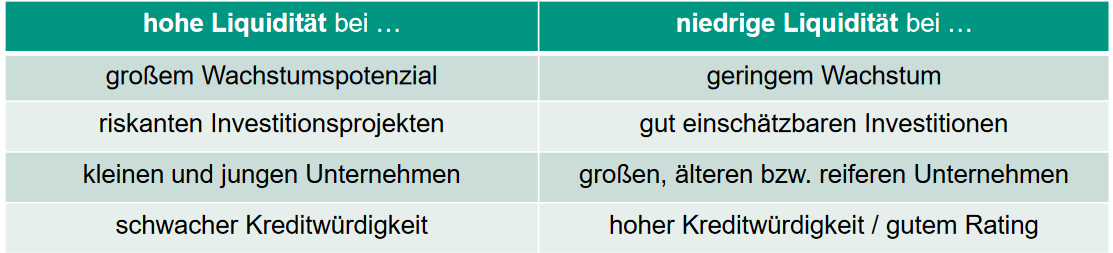
\includegraphics[width=0.7\textwidth]{images/e3.png}
\end{center}
\pagebreak

\subsection{Baumol-Modell} 
Kassenhaltung ist ein Abwägen zwischen Opportunitäts- und Transaktionskosten

\textbf{Annahmen}:
\begin{itemize}
	\item deterministisch
	\item keine Zahlungseingänge während der Periode
	\item konstante Auszahlungsrate
	\item keine Transaktionszeit $\ldots$
\end{itemize}

\textbf{Notation}:
\begin{itemize}
	\item $i$ = Rendite marktfähiger Wertpapiere ($\rightarrow$ Opportunitätskosten)
	\item $F$ = fixe Transaktionskosten für Wertpapierverkauf
	\item $T$ = Gesamtbedarf an Zahlungsmitteln innerhalb der
	Planungsperiode
	\item $C$ = Menge an Bargeld je Order
\end{itemize}
\begin{center}
	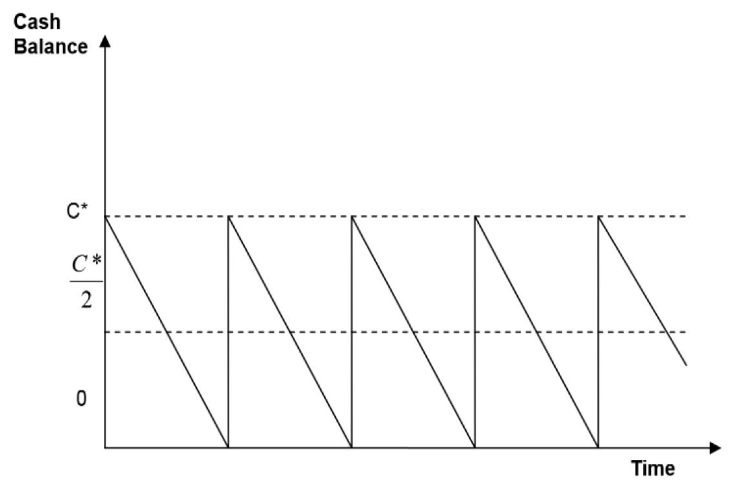
\includegraphics[width=0.6\textwidth]{images/e4.png}
\end{center}
\begin{itemize}
	\item Kosten = Opportunitätskosten + Transaktionskosten
	\item Opportunitätskosten $=i\cdot\frac{C}{2}$ (Opportunitätskosten $\cdot$ Durchschnittlicher Kassenbestand)
	\item Transaktionskosten $=F\cdot\frac{T}{C}$ (Transaktionskosten $\cdot$ Anzahl Transaktionen)
	\item \textbf{Optimale Höhe der Bargeldorder} $C^*=\sqrt{\frac{2\cdot T\cdot F}{i}}$
	\item Maximaler Kassenbestand = $C^*$
	\item Anzahl Transaktionen $=\frac{T}{C}$
\end{itemize}